\documentclass{article}
\usepackage{xparse}
\usepackage{graphicx}
\usepackage{float}
\usepackage[T1]{fontenc}

\title{SafeStreets}
\author{Marco Premi, Fabrizio Siciliano, Giuseppe Taddeo}
\pagestyle{headings}

\begin{document}
\maketitle

\tableofcontents

\newpage
\section{Introduction}
\subsection{Purpose}
\subsubsection{General Purpose}
    The purpose of this document is to correctly analyze all requirements, goals
    and actions needed in order to correctly develop SafeStreets.\\
    \\
    SafeStreets is a crowd-sourced application that intends to provide users
    with the possibility to notify authorities when traffic violations occur
    (eg. traffic violations) and will help to maintain stability and order
    within the streets. A reporting system will also be available to police
    offices and municipality employees in order to allow them to analyze (and
    take actions accordingly) different areas of the city and assess which areas
    have the most violations committed in.\\
    \\
    The core application will focus on storing useful traffic violation data
    provided by users, mainly with the help of input forms and hard evidence
    such as images. At any violation input, SafeStreets will also store useful
    metadata such as date and time the violation was retrieved, geolocate where
    it is and update a city wide map highlighting the areas where violations
    happen.\\
    \\
    In addition to that, with the help of third parties (eg. municipality),
    SafeStreets will be able to retrieve the data given by such party and
    cross-reference them with its own data retrieved by users. By doing so, it
    will be possible to identify unsafe areas, assess which kind of problems
    happen more frequently and suggest possible intervention. It will also be
    possible for third parties (municipality and police officers) to
    automatically generate traffic tickets. This will be happening in order to
    cross-reference all available data in order to build statistics such as the
    most (or less) egregious offenders or the effectiveness of the SafeStreets
    initiative \subsubsection{Goals} Follows a list of all goals that will be
    reached with the SafeStreets initiative.
    \begin{itemize}
        \item G1: The system must allow all kind of users (both third parties
        and civilians) to correctly input (with hard evidence) traffic
        violations around the city;
        \item G2: The system must autonomously retrieve metadata from hard
        evidence useful to report and to all users;
        \item G3: The system must allow to create different clearance levels in
        order to offer different reporting systems to different kind of users;
        \item G4: The system will provide an efficient reporting system in order
        to highlight different violation categories through all parts of the
        city where the initiative is active;
    \end{itemize}
\subsection{Scope}
With SafeStreets users can notify the authorities when traffic violations occur,
and in particular parking violations. Both user and authorities must register to
the application and agree that SafeStreets stores the information provided,
completing it with suitable meta-data. The whole system, because it tracks users
information, must respect the standards defined for processing of sensitive
information such as GDPR if it is used in Europe. The user sends the type of the
violation to the municipality and direct proofs of it (like a photograph). The
system runs an algorithm to read the license plate and also asks the user to
directly insert the license for a better recognition. Of course other
information are required, like the name of the street when the violation has
occurred, which can be retrieved from user's direct input or from the
geographical position of the violation (using Google Maps API). Both users and
authorities can highlight the streets with the highest frequency of violations
or the vehicles that commit the most violations. SafeStreets crosses information
about the accidents that occur on the territory of the municipality with his own
data to identify potentially unsafe areas and suggest possible interventions.
Because municipality could generates traffic tickets from the information about
violations SafeStreets should guarantee that information is never altered (if a
manipulations occurs, the application should discard the information). Such
features are made possible trough the use of two mobile applications(one for the
citizens and one for the officers on the field). The collected information are
sent to a back-end. All the services can also be accessed through a specific
web-site. 
\subsection{Definitions, Acronyms, Abbreviations}
\subsubsection{Definitions}
\paragraph{User:} it is identified as a civilian customer of the product. It
will be the main source for the SafeStreets initiative to obtain information
about traffic violations and therefore be successful; \paragraph{Third
parties:}those kind of organization/company that could provide services useful
to SafeStreets and that will be able to retrieve data in order to improve the
streets' safety; \paragraph{Customer:} it defines both third party SafeStreets
users (police officers or municipality employees) and civilians;
\paragraph{Ghiro:} image manipulation detection software, used by third party
users in order to detect any image manipulation and assess the veracity of the
hard evidence connected to the traffic ticket
\subsubsection{Acronym}
\paragraph{UI:} User Interface \paragraph{GDPR:} General Data Protection
Regulation \paragraph{API:} Application Programming Interface \paragraph{GPS:}
Global Positioning System
\subsubsection{Abbreviations}
\paragraph{Gn:} nth goal; \paragraph{Dn:} nth domain; \paragraph{Rn:} nth
requirement;
\subsection{Revision History}
\subsection{Reference Documents}
\subsection{Document Structure}
\paragraph{Chapter 1 - Introduction}
Gives an introduction to the problem by describing the purpose of SafeStreets.
It also shows the goals and the scope of the application. \paragraph{Chapter 2 -
Overall Description}[H] Offers an overall description of the project. It
identifies the actors involved in the application and lists all the assumptions
in order to identify all the boundaries of the project. The product perspective
includes details on the shared phenomena and the domain models. The class
diagram describe the domain model used and the state diagrama analyzes:
\begin{itemize}
    \item The process of collecting violations from users
    \item The process of sharing informations with the municipality
\end{itemize}
The majority of functions of the system are more precisely specified by taking
in mind the goals of the system.  
\paragraph{Chapter 3 - Specific Requirements}
Contains external interface requirements which are: user interfaces, hardware
interfaces, software interfaces and communication interfaces. Few scenarios
describing how the system acts in real world are listed here. Furthermore it
provides the description of the functional requirements, through the use of use
cases and sequence diagrams. The non-functional requirements are defined through
performance requirements, design constraints and software system attributes.
\paragraph{Chapter 4 - Formal analysis using Alloy}
Includes the alloy model of some critical aspects with comments and
documentation.
\paragraph{Chapter 5 - Effort Spent}
Shows the effort spent by each single group member while working on the RASD.
\paragraph{Chapter 6 - References}
Includes the documents we used as reference.

\newpage
\section{Overall Description}
\subsection{Product Perspective}
SafeStreets is designed to be a completely new software applications. It uses
some already proven services (Google Maps, PlateRecognizer APIs and Ghiro
software) for its critical tasks. The software uses these services in order to
double check whether both addresses and license plates are correctly
standardized in order to be stored into the violations database and if the
collected hard evidence have been somehow manipulated or corrupted.\\
The system is composed of two different mobile applications: one for the
citizens that want to reports violations and one for the officers acting on the
field. It also provides a web site for third party users which allows them to
assess and analyze potential unsafe areas, thanks also to a powerful reporting
system.\\
Taken into consideration that the municipality could generate traffic tickets
from the input violations, the software will be critical when it comes to
handling chain of custody. The latter is assured to never be broken by not
allowing any kind of customer (user, PO or employee) to modify the reported
violation. Supposedly, when some traffic violations might be erroneous or do not
have any reason of existence, the inputting user can warn the responsible third
party by attaching a warning explaining why it should not be taken into
consideration. The systems also ensures the veracity of each violation and the
hard evidence attached to it by running a image manipulation detection software
(Ghiro, per instance). This process is used by third parties before the emission
of each ticket to the corresponding offender.\\
\\
A high-level class diagram can be found below, which provides a model of the
application domain. The most important classes (not all of those which will be
implemented once the software will be ready) are shown in order to define how
the different components of SafeStreets will be communicating with each other.
It is possible to identify two kinds of third party users: police officers and
municipality employees. The first ones will be given access to both mobile
application and web application; the latter will be provided access just to the
above mentioned web application which will help these users assess the veracity
of the hard evidence attached to the traffic violations and to further analyze
unsafe areas around the municipality.\\

\begin{figure}[H]
    \centering
    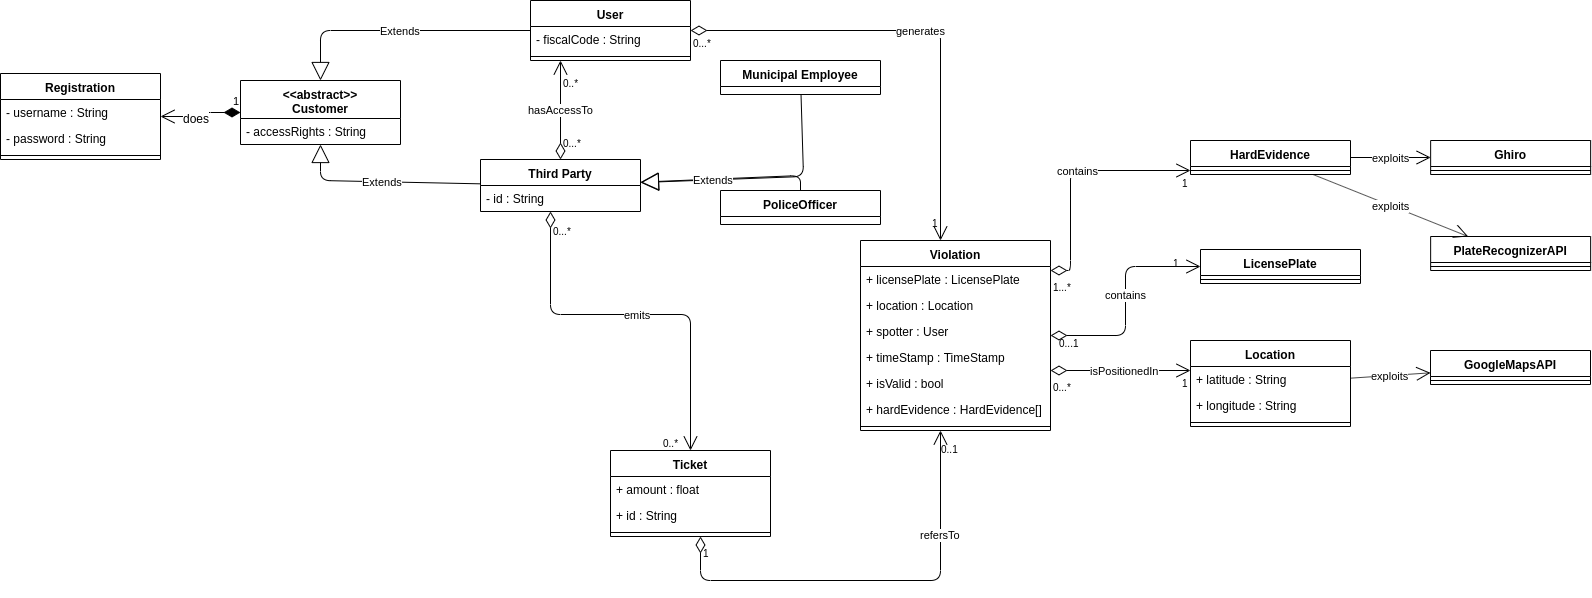
\includegraphics[scale=0.255]{Images/umlmodel}
    \caption{Class diagram}
\end{figure}

\subsection{Product Functions}
In the following section the most important product functions of the system are
reported.
%qua vanno aggiunte le varie funzioni
\subsection{User characteristics}
\subsection{Assumptions, dependencies and constraints}
\subsubsection{Assumptions}
\subsubsection{Dependencies}
\subsubsection{Constraints}

\newpage
\section{Specific Requirements}
\subsection{External Interface Requirements}
\subsubsection{User Interfaces}
\begin{figure}[H]
    \centering
    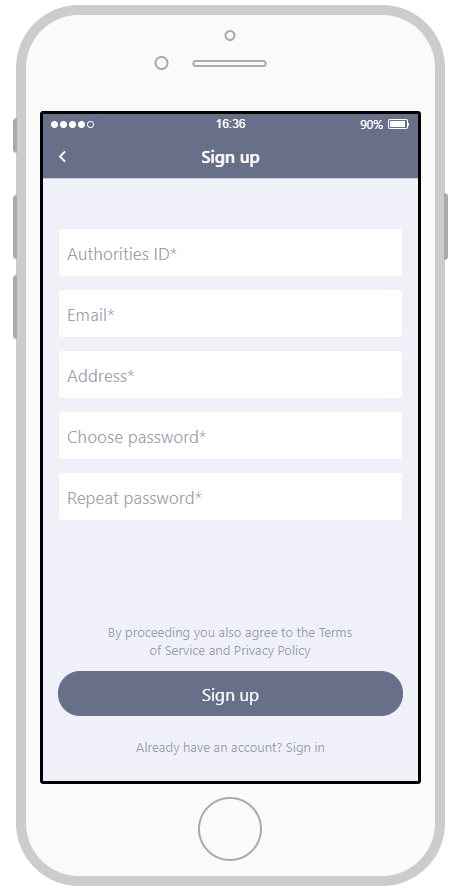
\includegraphics[scale=0.7]{Images/SignUpAuthoritiesApp}
    \caption{SignUp authorities}
\end{figure}
\begin{figure}[H]
    \centering
    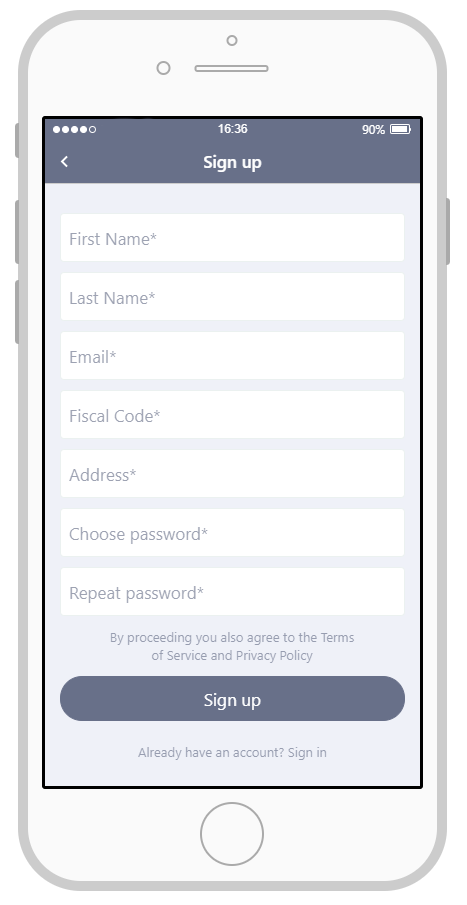
\includegraphics[scale=0.7]{Images/SignUpUtenteAPP}
    \caption{SignUp User}
\end{figure}
\begin{figure}[H]
    \centering
    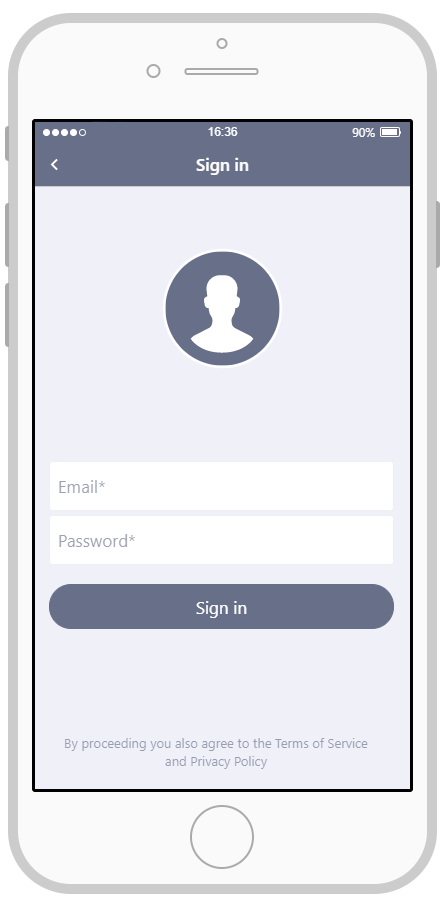
\includegraphics[scale=0.7]{Images/SignInAPP}
    \caption{SignIn}
\end{figure}
\begin{figure}[H]
    \centering
    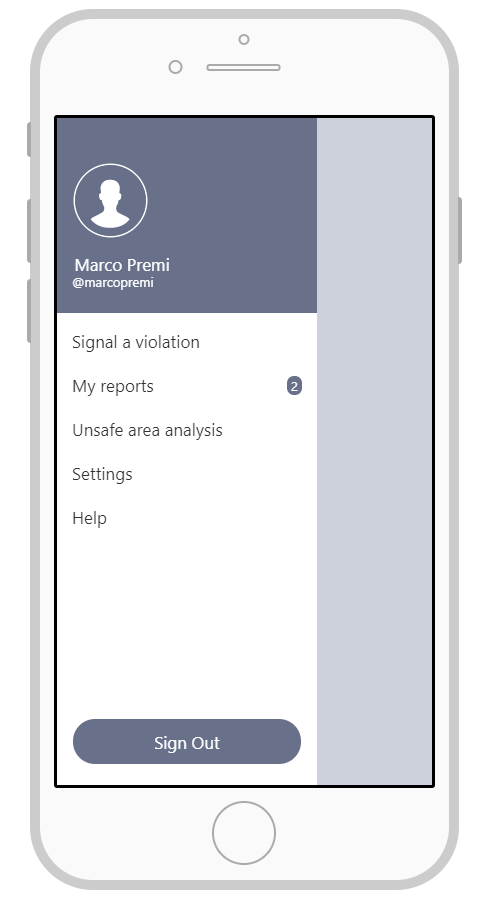
\includegraphics[scale=0.7]{Images/MenuAPP}
    \caption{Menu}
\end{figure}
\begin{figure}[H]
    \centering
    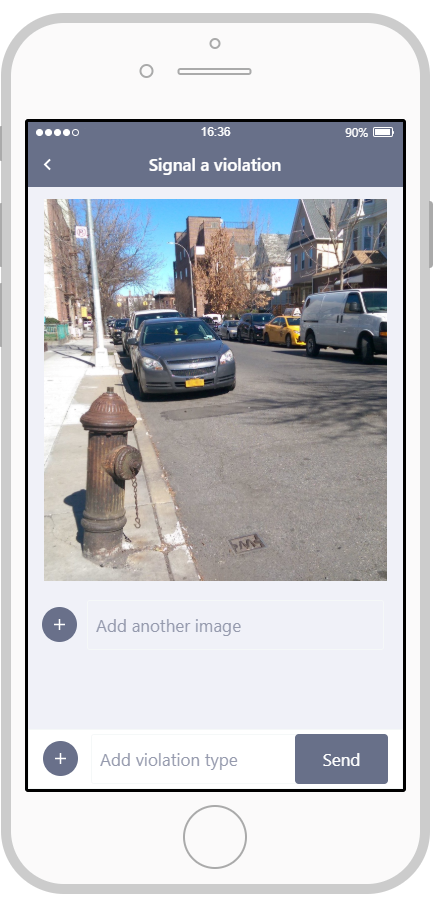
\includegraphics[scale=0.7]{Images/SignalAViolationAPP}
    \caption{SignIn}
\end{figure}
\begin{figure}[H]
    \centering
    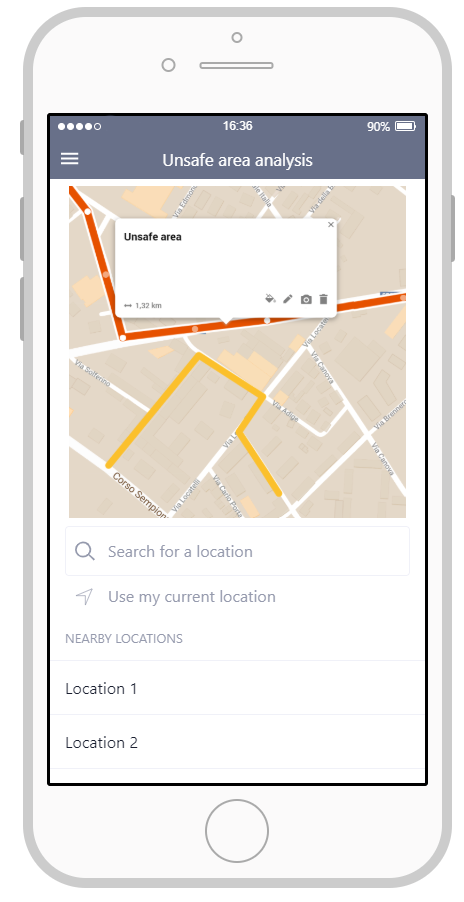
\includegraphics[scale=0.7]{Images/UnsafeAreaAnalysisAPP}
    \caption{SignIn}
\end{figure}
\begin{figure}[H]
    \centering
    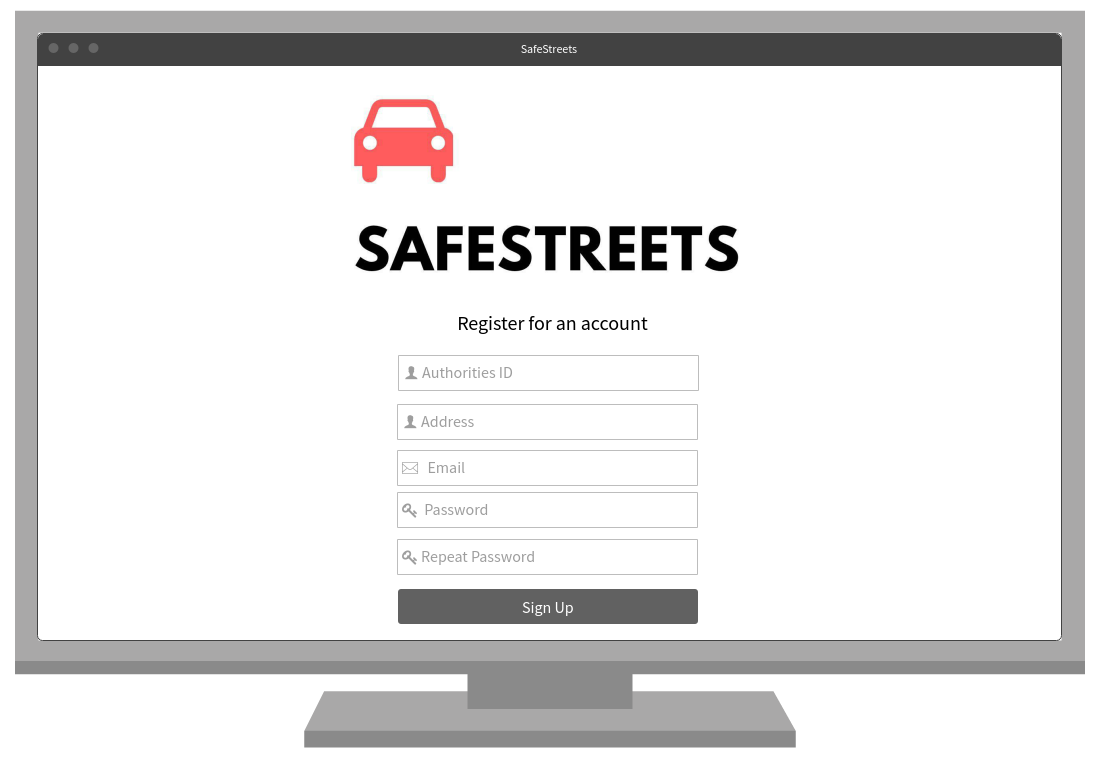
\includegraphics[scale=0.35]{Images/WEBSignUp}
    \caption{SignUp}
\end{figure}
\begin{figure}[H]
    \centering
    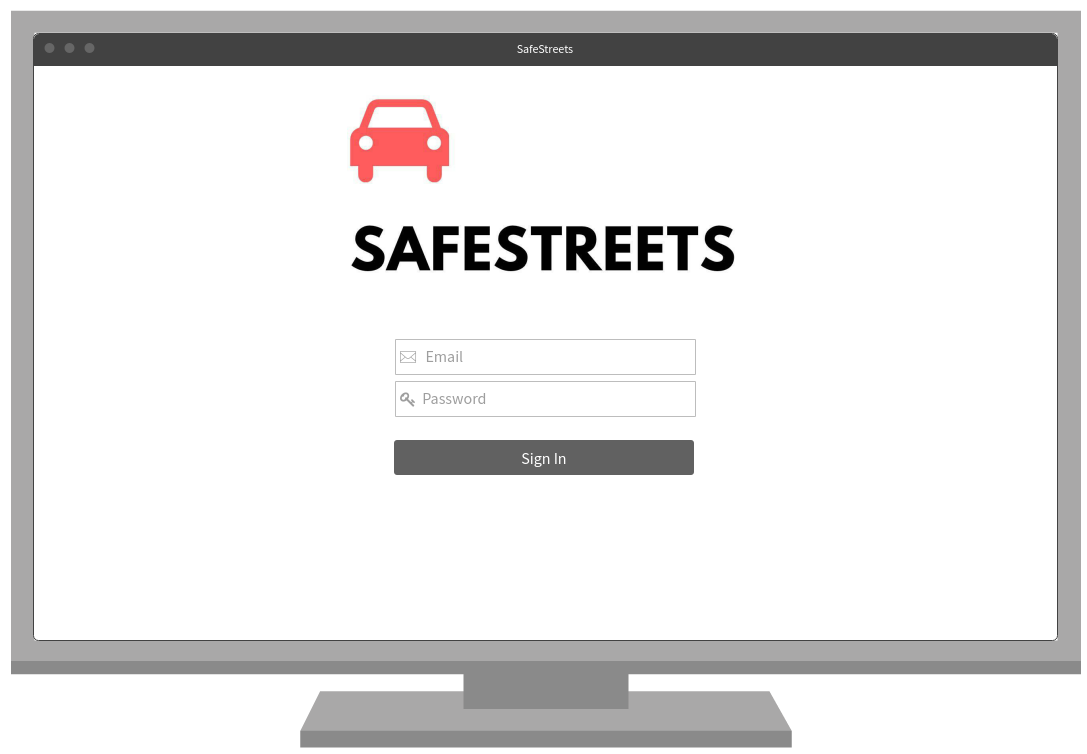
\includegraphics[scale=0.35]{Images/WEBSignIn}
    \caption{SignIn}
\end{figure}
\begin{figure}[H]
    \centering
    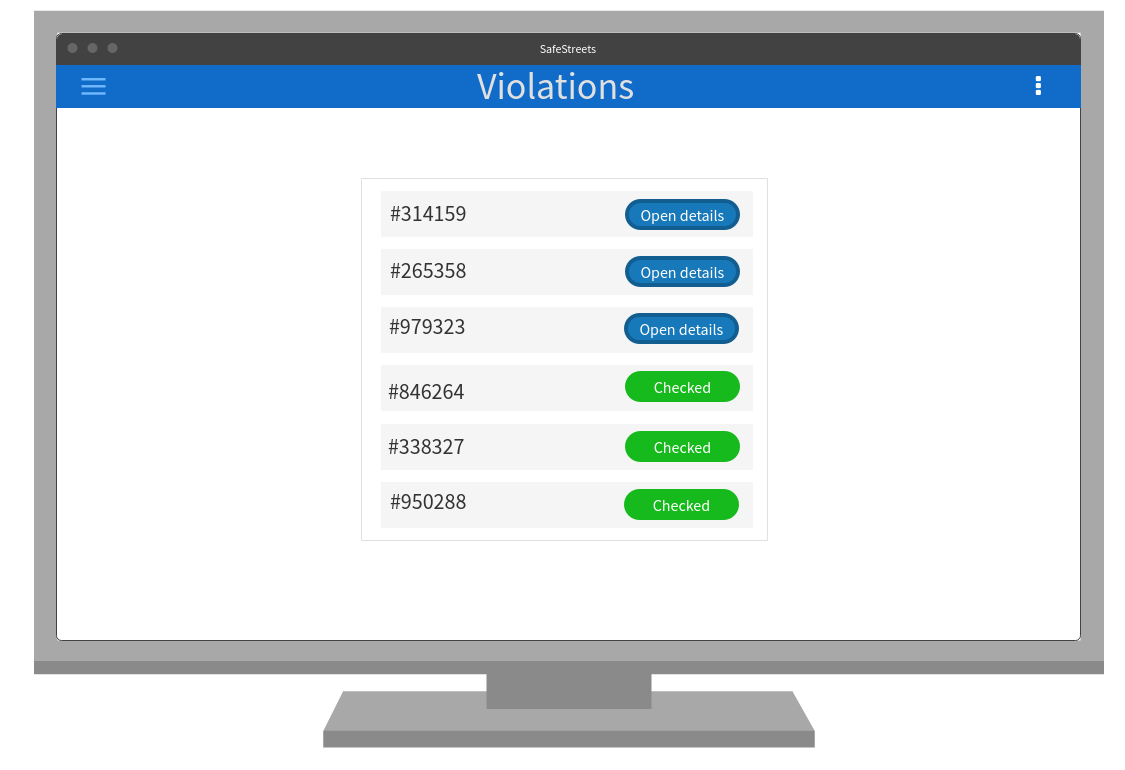
\includegraphics[scale=0.35]{Images/WEBViolations}
    \caption{Violations}
\end{figure}
\begin{figure}[H]
    \centering
    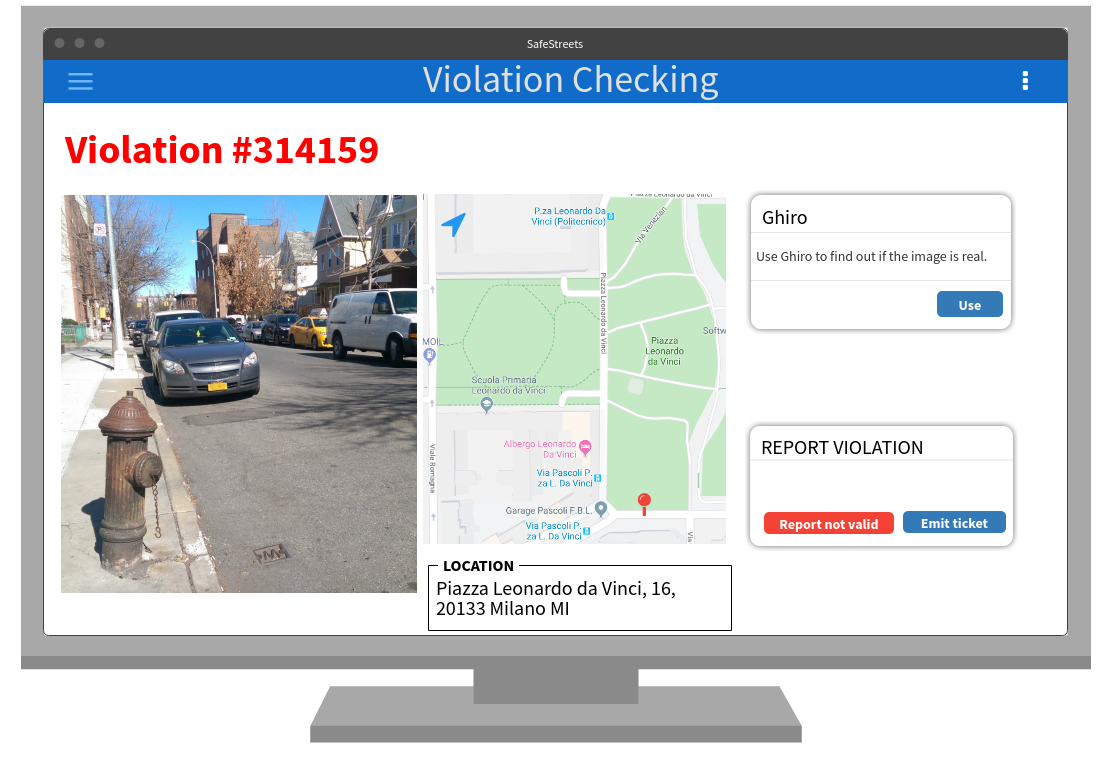
\includegraphics[scale=0.35]{Images/WEBViolationChecking}
    \caption{Violations checking}
\end{figure}
\begin{figure}[H]
    \centering
    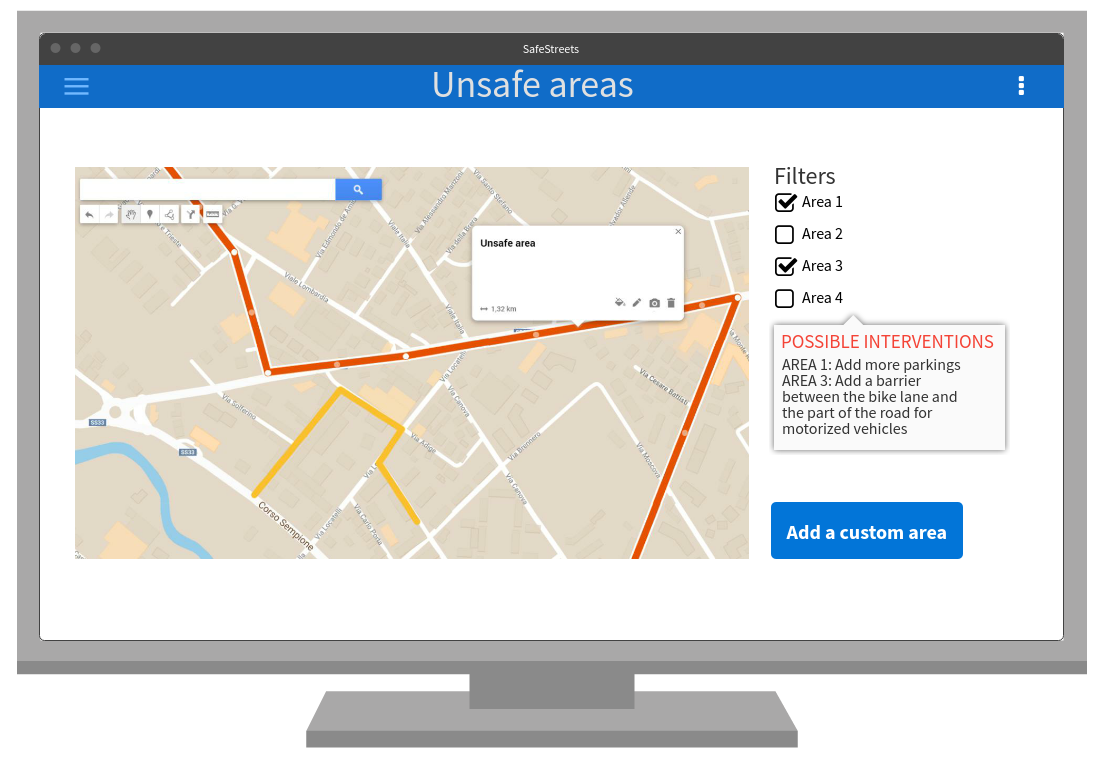
\includegraphics[scale=0.35]{Images/WEBUnsafeAreas}
    \caption{Unsafe Areas}
\end{figure}
\newpage
\newpage
\subsubsection{Hardware Interfaces}
The system has no hardware interfaces.
\subsubsection{Software Interfaces}
The system doesn't provide any API to external applications.\\
However some softwares part of SafeStreets is developed by other companies.
\begin{itemize}
    \item Google Maps API: for localization and creation of unsafe areas.
    \item Plate Recognizer API: for License Plate recognition.
    \item Ghiro: a digital image forensics tool used for find out if the image
    in the violation report is real.
\end{itemize}
\subsubsection{Communication Interfaces}
The system only uses HTTP(more precisely HTTPS) as communication service.
HTTP/HTTPS is used for:
\begin{itemize}
    \item User and third parties registration.
    \item Sending violations both to SafeStreets and to authorities.
    \item Using Google Maps API and Plate Recognizer API
\end{itemize}
\subsection{Scenarios}
\subsection{Functional requirements}
\paragraph{User}\mbox{}\\
$\langle$\textbf{G0}$\rangle$ SignUp to the system
\begin{description}
    \item $\langle$\textbf{R1}$\rangle$ the user must not be already registered
    in the system with the same email or fiscal code
    \item $\langle$\textbf{R2}$\rangle$ fiscal code and email must be valid and
    belonging to the user who is signing up
    \item $\langle$\textbf{R3}$\rangle$ the system must verify her/his email
    \item $\langle$\textbf{R4}$\rangle$ the user must agree to the Term of Use
\end{description}\mbox{}\\
$\langle$\textbf{G1}$\rangle$ SignIn to the system
\begin{description}
    \item $\langle$\textbf{R5}$\rangle$ the user must already be registered in
    the system
    \item $\langle$\textbf{R6}$\rangle$ the user must insert her/his email and
    the password \end{description}\mbox{}\\\\
$\langle$\textbf{G}$\rangle$ Signal a violation
\begin{description}
    \item $\langle$\textbf{R}$\rangle$ the user must be able to insert one or
    more photos of the violation
    \item $\langle$\textbf{R}$\rangle$ the user must send information about his
    location
    \item $\langle$\textbf{R}$\rangle$ the user can add more informations about
    the violation
\end{description}
%una volta inserita la violazione nessuno può cambiarla
$\langle$\textbf{G}$\rangle$ Show Unsafe Areas
\begin{description}
    \item $\langle$\textbf{R}$\rangle$ the user is shown the unsafe areas around
    him
    \item $\langle$\textbf{R}$\rangle$ the user is allowed to filter the unsafe
    areas
    \item $\langle$\textbf{R}$\rangle$ the user is allowed to search unsafe
    areas 
\end{description}    
$\langle$\textbf{G}$\rangle$ Manage Account
\begin{description}
    \item $\langle$\textbf{R}$\rangle$ the user must be able to change his/her
    address, the password and the email
    \item $\langle$\textbf{R}$\rangle$ the user must be able to delete his/her
    account
\end{description}

\paragraph{Third parties}\mbox{}\\
$\langle$\textbf{G}$\rangle$ SignUp to the system
\begin{description}
    \item $\langle$\textbf{R}$\rangle$ the third party must have a valid
    AuthoritiesID
    \item $\langle$\textbf{R}$\rangle$ the third party must not be already
    registered  in the system
    \item $\langle$\textbf{R}$\rangle$ the third party must supply a valid
    institutional email
    \item $\langle$\textbf{R}$\rangle$ must agree to the Term of Use
\end{description}\mbox{}\\
$\langle$\textbf{G}$\rangle$ SignIn to the system
\begin{description}
    \item $\langle$\textbf{R}$\rangle$ the third party must be already sign up
    \item $\langle$\textbf{R}$\rangle$ the third party must insert the email and
    the password\\
\end{description}
$\langle$\textbf{G}$\rangle$ Check Violations
\begin{description}
    \item $\langle$\textbf{R}$\rangle$ the third party must be able to check all
    the new and past violations
    \item $\langle$\textbf{R}$\rangle$ the third party must be able to use Ghiro
    \item $\langle$\textbf{R}$\rangle$ the third party must be able to report if
the violation is valid or not \end{description}\mbox{}\\
$\langle$\textbf{G}$\rangle$ Create Unsafe Areas
\begin{description}
    \item $\langle$\textbf{R}$\rangle$ the third party must be able to create
    and delete unsafe areas
    \item $\langle$\textbf{R}$\rangle$ the third party must be able to filter
    the different unsafe areas
\end{description}    



\subsection{Use Cases}
\subsubsection{User use cases}
%inizio prototipo tabella
\begin{table}[H]
    \begin{tabular}{|l|l|}
    \hline
    Name & \begin{minipage}[t]{0.7\textwidth}\textbf{} \end{minipage} \\ \hline  
    Actor & \begin{minipage}[t]{0.7\textwidth} \end{minipage} \\ \hline 
    Entry conditions & \begin{minipage}[t]{0.7\textwidth} \end{minipage} \\
    \hline 
    Events flow & \begin{minipage}[t]{0.7\textwidth} \end{minipage} \\ \hline
    Exit conditions & \begin{minipage}[t]{0.7\textwidth} \end{minipage} \\
    \hline
    Exceptions & \begin{minipage}[t]{0.7\textwidth} \end{minipage} \\ \hline
    \end{tabular}
\end{table}
%fine prototipo tabella 

\begin{table}[H]
    \begin{tabular}{|l|l|}
    \hline
    Name & \textbf{Sign Up} \\ \hline  
    Actor & User\\ \hline 
    Entry conditions &  The user has downloaded the application on his/her
    device\\ \hline 
    Events flow & 
    \begin{minipage}[t]{0.7\textwidth}
    \begin{enumerate}
        \item The user opens the application on his/her device
        \item The user clicks on "Sign Up" button
        \item The user fills the registration form with all the mandatory fields
        \item The user clicks the confirmation button
        \item The system saves the data
    \end{enumerate}
    \end{minipage} \\ \hline
    Exit conditions & \begin{minipage}[t]{0.7\textwidth}The system has stored
    user data, the user is registered and now is able to use te application
    \end{minipage}\\ \hline
    Exceptions & \begin{minipage}[t]{0.7\textwidth} \begin{enumerate}
        \item The user was already signed up
        \item The user doesn't fill all the mandatory fields with valid data
        \item The email or the fiscal code is already registered
        \item The user closes the application before the process has ended
    \end{enumerate}\end{minipage} \\ \hline
    \end{tabular}
\end{table}

\begin{table}[H]
    \begin{tabular}{|l|l|}
    \hline
    Name &\begin{minipage}[t]{0.7\textwidth} \textbf{Sign In} \end{minipage} \\ \hline  
    Actor & \begin{minipage}[t]{0.7\textwidth} User \end{minipage} \\ \hline 
    Entry conditions & \begin{minipage}[t]{0.7\textwidth} \begin{enumerate}
        \item The user has already downloaded the the application on his/her
        device
        \item The user has already signed up
    \end{enumerate}
    \end{minipage} \\ \hline 
    Events flow & \begin{minipage}[t]{0.7\textwidth}
    \begin{enumerate}
        \item The user opens the application on his/her device
        \item The user inserts his/her credentials in the "Email" and "Password"
        fields.
        \item The user clicks on the "Sign In" button
    \end{enumerate}
    \end{minipage} \\ \hline
    Exit conditions & \begin{minipage}[t]{0.7\textwidth} The user is
    successfully signed in \end{minipage} \\ \hline
    Exceptions & \begin{minipage}[t]{0.7\textwidth}
    \begin{enumerate}
        \item The user inserts invalid Email
        \item The user inserts invalid Password   
        \item The user closes the application before the process has ended 
    \end{enumerate}
    \end{minipage} \\ \hline
    \end{tabular}
\end{table}

\begin{table}[H]
    \begin{tabular}{|l|l|}
    \hline
    Name & \begin{minipage}[t]{0.7\textwidth} \textbf{Signal a violation}\end{minipage}
    \\ \hline  
    Actor & \begin{minipage}[t]{0.7\textwidth} User\end{minipage} \\ \hline 
    Entry conditions & \begin{minipage}[t]{0.7\textwidth} The user has already
    logged in \end{minipage} \\ \hline 
    Events flow & \begin{minipage}[t]{0.7\textwidth}
    \begin{enumerate}
        \item The user opens the Menu
        \item The user click on "Signal a violation" button in the Menu
        \item The user uploads one or more photos
        \item The user adds additional information
        \item The user adds one or more violation types
        \item The user clicks "Send"
        \item SafeStreets receives the violation
    \end{enumerate}
    \end{minipage} \\ \hline
    Exit conditions & \begin{minipage}[t]{0.7\textwidth}The user has
    successfully reported a violation \end{minipage} \\ \hline
    Exceptions & \begin{minipage}[t]{0.7\textwidth}
    \begin{enumerate}
        \item The user closes the application before the process has ended 
        \item The user doesn't have internet connection 
    \end{enumerate}    
    \end{minipage} \\ \hline
    \end{tabular}
\end{table}


\begin{table}[H]
    \begin{tabular}{|l|l|}
    \hline
    Name & \begin{minipage}[t]{0.7\textwidth} \textbf{Visualize unsafe areas} \end{minipage} \\ \hline  
    Actor & \begin{minipage}[t]{0.7\textwidth} User \end{minipage} \\ \hline 
    Entry conditions & \begin{minipage}[t]{0.7\textwidth} The user has already
    logged in\end{minipage} \\
    \hline 
    Events flow & \begin{minipage}[t]{0.7\textwidth} 
    \begin{enumerate}
        \item The user opens the Menu
        \item The user clicks on the "Unsafe area analysis" button in the Menu
        \item The user is allowed to select different filters and the area
        he/she wants to see
    \end{enumerate}
    \end{minipage} \\ \hline
    Exit conditions & \begin{minipage}[t]{0.7\textwidth} The user can see all
    the unsafe areas proposed by SafeStreets and the third party\end{minipage}
    \\
    \hline
    Exceptions & \begin{minipage}[t]{0.7\textwidth}  The user doesn't have
    internet connection \end{minipage} \\ \hline
    \end{tabular}
\end{table}

\begin{table}[H]
    \begin{tabular}{|l|l|}
    \hline
    Name & \begin{minipage}[t]{0.7\textwidth} \textbf{Visualize previous reports}\end{minipage} \\ \hline  
    Actor & \begin{minipage}[t]{0.7\textwidth} User\end{minipage} \\ \hline 
    Entry conditions & \begin{minipage}[t]{0.7\textwidth} The user has already
    logged in \end{minipage} \\
    \hline 
    Events flow & \begin{minipage}[t]{0.7\textwidth} 
    \begin{enumerate}
        \item The user opens the Menu
        \item The user selects the "My reports" button in the Menu
        \item The user is allowed to see all the previous reports he/she made
    \end{enumerate}    
    \end{minipage} \\ \hline
    Exit conditions & \begin{minipage}[t]{0.7\textwidth} The user is provided
    with the requested data \end{minipage} \\
    \hline
    Exceptions & \begin{minipage}[t]{0.7\textwidth} The user doesn't have
    internet connection  \end{minipage} \\ \hline
    \end{tabular}
\end{table}

\begin{table}[H]
    \begin{tabular}{|l|l|}
    \hline
    Name & \begin{minipage}[t]{0.7\textwidth} \textbf{Manage Account} \end{minipage} \\ \hline  
     Actor & \begin{minipage}[t]{0.7\textwidth} User \end{minipage} \\ \hline 
     Entry conditions & \begin{minipage}[t]{0.7\textwidth} The user has already logged in \end{minipage} \\
     \hline 
     Events flow & \begin{minipage}[t]{0.7\textwidth} 
    \begin{enumerate}
        \item The user opens the Menu
        \item The user selects the "Settings" button in the Menu
        \item The user is allowed to change his/her adress, the password, the
        email or to delete the account
    \end{enumerate}    
    \end{minipage} \\ \hline
     Exit conditions & \begin{minipage}[t]{0.7\textwidth} New user settings are
     saved to his/her account or the account is deleted \end{minipage} \\
     \hline
     Exceptions & \begin{minipage}[t]{0.7\textwidth} The user closes the
     application before the process has ended \end{minipage} \\ \hline
    \end{tabular}
\end{table}

\subsubsection{Third party use cases}
\begin{table}[H]
    \begin{tabular}{|l|l|}
    \hline
     Name & \begin{minipage}[t]{0.7\textwidth}\textbf{Sign Up}\end{minipage} \\ \hline  
     Actor & \begin{minipage}[t]{0.7\textwidth} Third party\end{minipage} \\ \hline 
     Entry conditions & \begin{minipage}[t]{0.7\textwidth} The third party is
     not already registered\end{minipage} \\
     \hline 
     Events flow & \begin{minipage}[t]{0.7\textwidth} 
    \begin{enumerate}
        \item The third party accesses SafeStreets website
        \item The third party is asked to sign in
        \item The third party clicks on "Sign Up"
        \item The third party fills the registration form with all the mandatory
        fields
        \item The third party clicks the confirmation button
        \item The system saves the data
    \end{enumerate}
    \end{minipage} \\ \hline
     Exit conditions & \begin{minipage}[t]{0.7\textwidth} The system has stored
     third party data, the third party is registered and now is able to use the
     website\end{minipage} \\
     \hline
     Exceptions & \begin{minipage}[t]{0.7\textwidth}
    \begin{enumerate}
        \item The third party was already signed up
        \item The third party doesn't fill all the mandatory fields with valid
        data
        \item The email or the AuthoritiesID is already registered
        \item The third party closed the application beforse the process has
        ended
    \end{enumerate}    
    \end{minipage} \\ \hline
    \end{tabular}
\end{table}

\begin{table}[H]
    \begin{tabular}{|l|l|}
    \hline
    Name & \begin{minipage}[t]{0.7\textwidth}\textbf{Sign In} \end{minipage} \\ \hline  
    Actor & \begin{minipage}[t]{0.7\textwidth} Third party \end{minipage} \\ \hline 
    Entry conditions & \begin{minipage}[t]{0.7\textwidth} The third party has already signed up\end{minipage} \\
    \hline 
    Events flow & \begin{minipage}[t]{0.7\textwidth}
    \begin{enumerate}
        \item The third party accesses SafeStreets website
        \item The third party is asked to sign in
        \item The third party inserts the credentials in the "Email" and
        "Password" fields.
        \item The third party clicks on "Sign In"
    \end{enumerate}    
    \end{minipage} \\ \hline
    Exit conditions & \begin{minipage}[t]{0.7\textwidth} The third party is successfully signed in \end{minipage} \\
    \hline
    Exceptions & \begin{minipage}[t]{0.7\textwidth}
    \begin{enumerate}
        \item The third party inserts invalid Email
        \item The third party inserts invalid Password
        \item The third party closes the website before the process has ended
    \end{enumerate}
    \end{minipage} \\ \hline
    \end{tabular}
\end{table}

\begin{table}[H]
    \begin{tabular}{|l|l|}
    \hline
    Name & \begin{minipage}[t]{0.7\textwidth}\textbf{Unsafe Areas} \end{minipage} \\ \hline  
    Actor & \begin{minipage}[t]{0.7\textwidth} Third party \end{minipage} \\ \hline 
    Entry conditions & \begin{minipage}[t]{0.7\textwidth} The third party has already logged in\end{minipage} \\
    \hline 
    Events flow & \begin{minipage}[t]{0.7\textwidth}
    \begin{enumerate}
        \item The third party clicks on the menu icon
        \item The third party click on "Unsafe ares"
        \item The third party is allowed create and delete unsafe areas, to
        select different filters and to search different areas
    \end{enumerate} 
    \end{minipage} \\ \hline
    Exit conditions & \begin{minipage}[t]{0.7\textwidth} The unsafe areas editor
    is presented to the third party\end{minipage} \\
    \hline
    Exceptions & \begin{minipage}[t]{0.7\textwidth} \end{minipage} \\ \hline
    \end{tabular}
\end{table}

\begin{table}[H]
    \begin{tabular}{|l|l|}
    \hline
    Name & \begin{minipage}[t]{0.7\textwidth}\textbf{Check Violations} \end{minipage} \\ \hline  
    Actor & \begin{minipage}[t]{0.7\textwidth} Third party \end{minipage} \\ \hline 
    Entry conditions & \begin{minipage}[t]{0.7\textwidth} The third party has already logged in \end{minipage} \\
    \hline 
    Events flow & \begin{minipage}[t]{0.7\textwidth}
    \begin{enumerate}
        \item The third party clicks on the menu icone
        \item The third party clicks on "Violations"
        \item The third party is allowed to see the list of previous and
        actual violations (checked or not)
        \item The third party click on "Open Details" of one particular not
        checked violation
        \item The third party is allowed to see information about the particular
        violation
        \item The third party can click "Use" on Ghiro card to find out if the
        image is real
        \item The third party can click "Report not valid" if the image is fake
        or "Emit Ticket" if the image is real
    \end{enumerate}
    \end{minipage} \\ \hline
    Exit conditions & \begin{minipage}[t]{0.7\textwidth} The third party can manage the violations \end{minipage} \\
    \hline
    Exceptions & \begin{minipage}[t]{0.7\textwidth}The third party closes the
    website before the process has ended \end{minipage} \\ \hline
    \end{tabular}
\end{table}

\begin{table}[H]
    \begin{tabular}{|l|l|}
    \hline
    Name & \begin{minipage}[t]{0.7\textwidth}\textbf{Manage Account} \end{minipage} \\ \hline  
    Actor & \begin{minipage}[t]{0.7\textwidth}Third party\end{minipage} \\ \hline 
    Entry conditions & \begin{minipage}[t]{0.7\textwidth} The third party has already logged in \end{minipage} \\
    \hline 
    Events flow & \begin{minipage}[t]{0.7\textwidth}
    \begin{enumerate}
        \item The third party clicks on the menu icon
        \item The third party click on "Manage Account"
        \item The third party is allowed to change the email, the password or to
        delete the account
    \end{enumerate}
    \end{minipage} \\ \hline
    Exit conditions & \begin{minipage}[t]{0.7\textwidth} New user settings are
    saved to the third party account or the account is deleted\end{minipage} \\
    \hline
    Exceptions & \begin{minipage}[t]{0.7\textwidth}The third party closes the
    website before the process has ended \end{minipage} \\ \hline
    \end{tabular}
\end{table}


\subsection{Performance requirements}
The system is provided to serve a great number of users and third parties
simultaneously. The back-end must be powerful enough to accept thousands of
requests at same time during all the day.\\
The front-end applications (mobile and web) don't have particular performance
requirements.
\subsection{Design Constraints}
\subsubsection{Standars compliance}
With regard to the privacy, security for the mobile application and the back-end
is a big issue, so the whole project is subject to the the GDPR. Furthermore
it's a good practice to apply W3C's Standards to ensure intercompatibility.
\subsubsection{Hardware Limitations}
Even if SafeStreets is a software-based service there are some hardware
limitations regarding the smartphones.
\begin{itemize}
    \item must be able to make HTTPS requests (connection to internet
    4G/3G/2G/Wi-Fi)
    \item must have on board GPS (mobile devices only)
\end{itemize}
\subsubsection{Any Other Constraint}
%probabilmente da cancellare (Secondo me non ci sono, a parere mio)
\subsection{Software System Attributes}
\subsubsection{Reliability}
The system must be able to run 24/7 without any interruptions. Only small
concessions from this requirement might be tolerated. The system must also be
fault tolerant. In order to exploit this last point the data saved on the
servers should be duplicated.
\subsubsection{Availability}
Maximum availability is a necessity because users should be able to report
violations 24/7. One or two days per year may be used for maintainance, so 
availability of 99\% is expected.
\subsubsection{Security}
User and third party provide data that contains sensitive information, so the
security aspect is of primary relevance.\\ Communications between user, third
party and SafeStreets must be encrypted and the database with all the data must
be protected from any possibile internal or external attack.
\subsubsection{Mantainability}
The system shoule be flexibile and easy to mantain. For this purpose the whole
system will be developed using a modular architecture. \\
Fixing and modifying the system will be easy with the modular architecture.

\subsubsection{Portability}
SafeStreets in order to be useful must be used by a very large number of people.
It is for this reason that third parties' registration website must be available
on the majority of browsers (Firefox, Google Chrome, Safari, Opera, Microsoft
Edge and Internet Explorer 11).\\
Naturally the mobile application must be available on both Android and iOs.

\newpage
\section{Formal Analysis using Alloy}

\newpage
\section{Effort spent}
\begin{center}
    \begin{tabular}{|c|c|c|c|c|}
        \hline
        \textbf{Description of the task} & \textbf{MP} & \textbf{FS} &
        \textbf{GT} \\
        Introduction                    & 2.5   & 2     & 0     \\
        Overall Description             & 3   & 3   & 0     \\
        Specific requirements           & 0     & 0     & 0     \\
        Formal analysis using Alloy     & 0     & 2     & 0     \\
    \end{tabular}
\end{center}
\section{References}
    \paragraph{Plate Recognizer:} https://app.platerecognizer.com
    
\end{document}  